\section{Velocity Profiler}

\subsection{Theory of Operation}

Velocity Profiler is responsible for generating a trajectory from the path segments provided by Path Planner.  Velocity Profiler is also responsible for keeping track of where the robot is in the computed trajectory. It provides the desired velocity based on the current desired trajectory to steering which then adds correction factors before it is finally sent to the robot's motors.

There were two methods of generating the trajectory, time based and
spatial based.  We chose to implement the spatially based method
because it made it easier to stop and resume the robot due to E-Stops
and obstacles in the path.

\subsubsection{Velocity Profiling Algorithm}

The current version of velocity profiler takes in segments published by the Path Planner in the form of a PathList message. This PathList message contains PathSegment specifications which give the position in space of path in small chunks. PathSegment messages also contain information about the constraints on that section of the path. Velocity profiler uses these constraints to compute things like the point in space to start and stop accelerating.

Each time a list of path segments is received, velocity profiler checks for changes in the segment number. Velocity profiler works under the assumption that the segment number is a unique id for a segment and that segment numbers will not decrease except in the event that a path is aborted. If a single segment has been changed then velocity profiler will recompute the trajectory. It would be difficult to recompute the trajectory for only the part that has changed because more segments then the ones that have changed can be affected by a change in a single segment. For instance if the minimum speed in a segment is raised it may mean that the next segment will need to immediately begin braking whereas before it may have accelerated. To avoid having to propagate effects of a single segment change throughout the entire trajectory velocity profiler simply starts from scratch each time it receives a segment.

In order to blend segments velocity profiler keeps track of the starting and ending velocity of each segment. Transitions between spin segments and lines and arcs require a full stop, but transitions between lines and lines, arcs and arcs, and arcs and lines can be blended together so that the robot may slow down, but it will not come to a complete halt.

Because of the structure of the velocity commands straight and spin commands can be profiled separately and each component can be controlled by velocity profiler to execute complex maneuvers. Arcs require that the spin trajectory be constrained to the speeds of the straight trajectory.

Velocity profiler uses an internal class called TrajSeg.  This class stores information about a single segment in the trajectory and provides a reference to the pathsegment instance to which it corresponds. This segment contains the type -- acceleration, deceleration, or constant velocity -- was well as stopping distance in terms of normalized segment length and start and stop velocities.  Using this information the velocity controller can execute a trajectory simply by looking at the next trajectory segment and using the information in it until its reached a point past the trajetory segment's stopping point.

To compute the trajectory segments the following basic kinematic equation is used:
\begin{center}
$v_f^2 = v_i^2 + 2*accel*dist$
\end{center}
Using this equation in the forward direction from the beginning of the segment velocity profiler can determine the stopping point of the acceleration portion of a path segment (if there is one). Using the equation in reverse starting from the end of the path, velocity profiler can determine the starting point of a deceleration segment and consequently the stopping point of a constant velocity segment.  If the starting point of the deceleration segment is before the stopping point of the acceleration segment there will be no constant velocity segment.

When calculating the acceleration stopping point if the result is negative then it means the final speed of the previous segment is faster than the maximum speed of the current segment and so the robot must actually start with a deceleration segment. Ideally this will never happen, however, it is difficult to check for this condition and its importance was not deemed high enough to justify the computation time. A similar thing can happen with the deceleration segment if the number comes out greater than 1.0 (the normalized path length). In that case the robot shouldn't decelerate, but neither can it accelerate without violating its maximum velocity constraint. In that case there will be no deceleration segment.

\subsubsection{State Class}
Velocity Profiler uses an internal class called State.  This class is
responsible for figuring out how far along the path the robot has
traveled.  This is used to determine when a segment is completed and
the next one should be loaded.

The first version simply integrated the velocity commands over time to
keep an internal belief state of where it is at. This caused problems because steering modified the velocity commands which made the internal belief state fall out of sync with reality.  To fix this we originally fed back in the steering commands that were actually sent to the robot. However, it was difficult to use. Instead because map position data is already available and the trajectory is already specified in terms of space points an entirely different algorithm was developed based on the geometry of the path segments.  Because each of the three segment types has a unique geometry each type of segment is dealt with differently.

\paragraph{Line Segments}
The lines work by assuming that the path segment is actually an infinitely long line. It then takes the robot's position and finds the line passing through this point and normal to the path segment line. The intersection of this line with the path segment line is found. The intersection points distance from the starting point of the path segment is then computed. Using the tangent angle of the path segment the state class determines if the point is before or after the starting point on the hypothetical line.  If the intersection point is before then the segment distance completed is negative otherwise it is positive. Also the segment distance completed is normalized with respect to path length meaning that numbers between 0.0 and 1.0 are within the specified path segment, numbers greater than 1.0 are past the end of the segment and numbers less than 0.0 are before the start of the segment.

\paragraph{Spin Segments}
The spins simply uses the orientation of the robot. The state class turns the initial tangent angle of the spin into a number between 0 and $2\pi$. It does the same for the orientation data. It then takes the difference between the current angle and the desired angle.  If the angle is positive then it will give a segment distance done greater than 0.0 and otherwise the number will be less than 0. There are some issues with wrap around on the unit circle.  To handle this I make sure all of the angles are referenced with respect to the 0 angle. Having a common reference means that I can tell where each angle is in relation to each other by referencing it with respect to the common reference. From there I transform the angles into a reference based on the initial tangent angle. This allows me to ignore wrap around of $2\pi$ to 0 on the unit circle.

There is a slight problem with this approach for the spins. Because of the wrap around it is necessary to specify a specific angle that will transition the segment distances done from negative to positives. To do this an angle halfway between the start and final angle of the spin segment is computed and $\pi$ is added to it. The problem with this approach is that the longer the spin in terms of radians the more likely it is the robot will skip over a number greater than 1.0 and cycle back around to a negative number. Also spins longer than $2\pi$ cannot be specified. This was not a real problem because we can split long segments into smaller ones and velocity profiler will blend them together.

\paragraph{Arc Segments}
The arcs are the most complicated, but share many similarities with the spin computations. The main difference is that the spins cannot have an offset from the center of the circle whereas the arcs can. For the arcs I start by finding the angle of the line from the robots current position to the specified arc's reference point. Originally the algorithm planned on looking for the intersection of this line segment with the circle that the arc would make were it long enough. However, the formula was difficult to compute and it was difficult to translate that point to a segment distance complete number like in the lines and spins algorithm. After finding the angle of the line between the robot and the arc's center all of the angles are converted to numbers between 0 and $2\pi$. This ensures that all the angles are referenced to the 0 angle making it far easier to compare where on the circle each angle is. The rest of the angle computations are the same as for the spin segment.

In order to test this algorithm a number of matlab scripts that plot the results of these calculations were written. These scripts made it easy to visualize the outcome of the computations and to see how the different parameters affected the outcome. An example image output is shown in figure ~\ref{fig:arcComputationExample}. In the figure the solid blue line is the specified arc segment, the dashed blue lines are the starting and final angles. The red dot on the blue line is the starting point. The magenta dot-dash line is the cutoff angle between negative and positive angles. The magenta x is the robot's position. The green dashed line is the line from the robot to the arc's reference point. The black x is the point on the circle that the line from the robot to the arc's reference point intersects the circle that a complete arc would specify.

\FloatBarrier

\begin{figure}[h]

  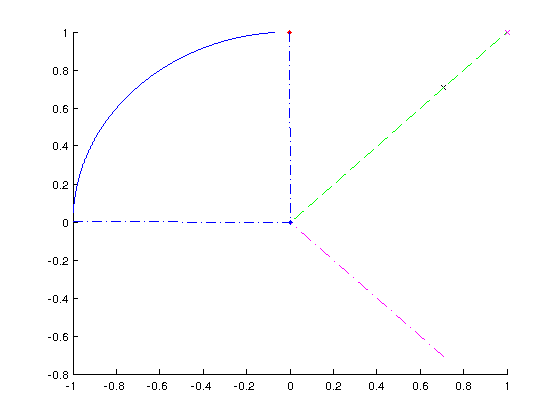
\includegraphics{images/arcComputationExample1.png}
  \caption{Robot at position (1,1,0) for an arc with curvature of 1.0, length of pi/2, starting angle of pi/2 and a center at (0,0,0). The segment distance completed is -0.5}
  \label{fig:arcComputationExample}
  
\end{figure}

\FloatBarrier

The code used to generate this figure is included in the report, but you can view the repository at \url{https://github.com/rhololkeolke/Velocity-Profiler-Simulations/}

\subsection{Observations}

We are using an AsyncSpinner to service our callbacks.  Using the
AsyncSpinner means we do not have to call spin or spinOnce, however,
it complicates the callbacks because now they are running on separate,
non-blocking threads.

During our testing we noticed that the information from single packets
would be lost.  We were testing Velocity Profiler with a dummy path
publisher node that published at a significantly slower rate than
velocity profiler's main loop.  Yet, the individual packets would
sometimes get skipped by velocity profiler's callback function.

We are still investigating the cause of this, but think it may have to
do with the use of AsynSpinner to service the callbacks.